\documentclass[a4paper,11pt]{article}
\usepackage{sbpo-template}
%\usepackage[latin1]{inputenc}
\usepackage[brazil]{babel}    % português do Brasil
\usepackage[utf8]{inputenc}   % acentos no UTF-8
\usepackage[T1]{fontenc}      % para hifenização correta
\usepackage{amsmath,amssymb,amsfonts}
\usepackage{url}
\usepackage[square]{natbib}
\usepackage{indentfirst}
\usepackage{fancyhdr}
\usepackage{graphicx}
\pagestyle{fancy}

\usepackage{hyperref}

\usepackage{tikz}
\usetikzlibrary{arrows.meta, positioning, fit, shapes.geometric}

\usepackage{placeins}
\usepackage{tabularx}
\usepackage{caption}
\usepackage{subcaption}
\usepackage{float}

\usepackage{mathrsfs}
\usepackage{multicol}
\usepackage{multirow}
\usepackage{booktabs}

\usepackage[square]{natbib}
\usepackage{indentfirst}
\usepackage{fancyhdr}
\usepackage{graphicx}
\usepackage{lscape}
\usepackage{empheq}
\usepackage{xcolor}
\usepackage{svg}
\usepackage{amsmath} 
% \usepackage[boxed, algoruled, linesnumbered, inoutnumbered]{algorithm2e}
\usepackage{algorithm}
\usepackage{algpseudocode}


\fancyhf{}
\fancyhead[C]{
\includegraphics[scale=0.5]{sbpo2026-header-logo.png}}
%\renewcommand{\headrulewidth}{0pt}
\renewcommand{\headruleskip}{-1mm}
%\setlength\headheight{101.0pt}
%\addtolength{\textheight}{-101.0pt}
\setlength\headheight{86pt}
\addtolength{\textheight}{-86pt}
\setlength{\headsep}{5mm}
\setlength{\footskip}{4.08003pt}

\begin{document}

\title{\textit{Matheuristica} Híbrida aplicada ao Problema de p-Medianas Capacitado} 

\maketitle
\thispagestyle{fancy}

\author{ 
\name{Gabriel Souto,  Luidi Simonetti, Pedro Henrique González}
\institute{Universidade Federal do Rio de Janeiro} 
\iaddress{R. Antônio Barros de Castro, 119 - Cidade Universitária, Rio de Janeiro - RJ, 21941-853}
\email {\{soutog,luidi,pegonzalez\}@cos.ufrj.br}
}

\vspace{8mm}
\begin{resumo}
O Problema das p-Medianas Capacitado (PPMC) é um problema NP-difícil aplicado em contextos de localização de facilidades, logística e planejamento de serviços, que busca selecionar instalações e alocar clientes minimizando custos de atendimento sob restrições de capacidade. Neste trabalho, propõe-se uma matheurística híbrida denominada \textit{Hybrid Clustering Search Adaptive Iterated Local Search} (Hybrid-CS-AILS), que combina estratégias de construção GRASP, busca local baseada em \textit{Variable Neighborhood Descent} (VND), um mecanismo adaptativo de \textit{Iterated Local Search} (AILS) e um procedimento de intensificação que utiliza um modelo exato através de \textit{Clustering Search}. Experimentos computacionais foram conduzidos em 35 instâncias benchmark clássicas do PPMC, comparando o método proposto com abordagens da literatura. Os resultados mostram que o Hybrid-CS-AILS obtém soluções competitivas em qualidade, em menor tempo computacional em relação aos métodos comparados, evidenciando a eficiência da estratégia híbrida proposta.
\end{resumo}

\bigskip
\begin{palchaves}
Problema das p-Medianas Capacitado; Matheurísticas; Clustering Search; Iterated Local Search; Otimização Combinatória; Localização de Facilidades.

% \bigskip
% \noindent{Tópicos: Metaheurísticas, Otimização Combinatória, Localização de Facilidades, Programação Matemática}
\end{palchaves}



\vspace{8mm}

\begin{abstract}
The Capacitated p-Median Problem (CPMP) is an NP-hard problem applied in facility location, logistics, and service planning contexts, which seeks to select facilities and allocate customers while minimizing service costs under capacity constraints. This work proposes a hybrid matheuristic called Hybrid Clustering Search Adaptive Iterated Local Search (Hybrid-CS-AILS), which combines GRASP construction strategies, local search based on Variable Neighborhood Descent (VND), an adaptive Iterated Local Search (AILS) mechanism, and an intensification procedure that uses an exact model through Clustering Search. Computational experiments were conducted on 35 classic benchmark instances of the CPMP, comparing the proposed method with approaches from the literature. The results show that Hybrid-CS-AILS achieves competitive solutions in terms of quality, with less computational time compared to the other methods, demonstrating the efficiency of the proposed hybrid strategy.
\end{abstract}

\bigskip
\begin{keywords}
Capacitated p-Median Problem; Matheuristics; Clustering Search; Iterated Local Search; Combinatorial Optimization; Facility Location.

% \bigskip
% \noindent{Paper topics (indicate in order of PRIORITY the paper topic(s))}
\end{keywords}

 
\newpage
\section{Introdução}

Problemas de localização de facilidades desempenham um papel central em diversos sistemas reais, incluindo logística urbana, planejamento de serviços de saúde, distribuição de recursos e redes de transporte \citep{drezner1996facility, revelle1996plant, owen1998strategic}. Nessas aplicações, decisões relacionadas à localização de instalações e à alocação de demanda impactam a eficiência operacional, os custos e a qualidade do serviço oferecido \citep{ullah2025optimizing}. 

Dentro desse contexto, o Problema das p-Medianas (PPM), originalmente introduzido por \cite{hakimi1964optimum}, destaca-se como um dos modelos fundamentais para problemas de localização e agrupamento. Este problema consiste, basicamente, em selecionar $p$ instalações (medianas) dentre um conjunto de candidatos e alocar os clientes a essas instalações, minimizando a soma das distâncias entre os clientes e suas respectivas medianas. Uma extensão desta modelagem original e de grande relevância prática é o Problema das p-Medianas Capacitado (PPMC), no qual cada instalação possui uma capacidade limitada de atendimento \citep{mulvey1984solving, pirkul1987efficient}.

Do ponto de vista computacional, o PPMC é um problema NP-difícil \citep{garey1990guide}, o que inviabiliza o uso de métodos exatos para instâncias de grande escala em tempo computacional condizente com aplicações práticas. Dessa forma, a literatura deste problema tem explorado o uso de heurísticas, metaheurísticas e, mais recentemente, matheurísticas para obter soluções de alta qualidade em tempos computacionais reduzidos.

Diversas abordagens têm sido propostas para o PPMC, incluindo métodos exatos baseados em branch-and-bound, branch-and-cut e geração de colunas \citep{mulvey1984solving, lorena2004column, boccia2008cut}, bem como abordagens inspiradas em metaheurísticas clássicas como GRASP, algoritmos genéticos, busca tabu e Variable Neighborhood Search (VNS) \citep{osman1994capacitated,correa2004genetic, diaz2006hybrid,fleszar2008effective}. Mais recentemente, abordagens híbridas, conhecidas como matheurísticas, têm se destacado ao combinar estratégias de busca com modelos de programação matemática, permitindo explorar de forma mais eficiente regiões do espaço de soluções conforme feito por  \cite{stefanello2015matheuristics}.

Apesar dos avanços recentes em matheurísticas para o PPMC, ainda permanece um desafio importante: decidir quando e onde aplicar mecanismos exatos de intensificação sem comprometer a eficiência computacional do método. Neste contexto, este trabalho propõe uma matheurística híbrida denominada Hybrid-CS-AILS, cuja principal contribuição é um mecanismo de intensificação seletiva orientado pela densidade de ótimos locais observados durante a busca. A proposta integra um Adaptive Iterated Local Search (AILS) \citep{lourencco2003iterated} com uma estratégia de Clustering Search \cite{oliveira2013clustering} capaz de identificar regiões promissoras do espaço de soluções. Deste modo, as principais contribuições deste trabalho são:

\begin{enumerate}
\item uma estratégia de intensificação guiada por densidade de ótimos locais obtidos durante a busca;

\item a integração entre Clustering Search e Adaptive Iterated Local Search como mecanismo de decisão para chamada de modelo de programação inteira mista;

\item um modelo baseado em subproblemas reduzidos adaptativamente definidos de acordo com o estado da busca;

\end{enumerate}

A estrutura deste artigo está organizada da seguinte forma: a Seção \ref{secRelated} apresenta os trabalhos relacionados; a Seção \ref{secDef} descreve o Problema das p-Medianas Capacitado e sua formulação matemática; a Seção \ref{secMet} detalha o método proposto e seus componentes; os experimentos computacionais e a análise dos resultados são apresentados na Seção \ref{secExp}; por fim, a Seção \ref{secCon} apresenta as conclusões e direções para trabalhos futuros.


\section{Trabalhos Relacionados}
\label{secRelated}

Desde sua proposição como extensão do problema clássico das p-medianas
\cite{hakimi1964optimum}, o PPMC tem sido estudado tanto por métodos
exatos quanto por abordagens heurísticas, motivado por aplicações em
planejamento de saúde, logística urbana e alocação de recursos
\citep{revelle1996plant, drezner1996facility}. Métodos exatos,
incluindo enumeração implícita~\cite{mulvey1984solving},
\textit{branch-and-cut} e geração de colunas
\cite{lorena2004column, ceselli2005branch, boccia2008cut}, garantem
otimalidade, mas têm custo computacional proibitivo em instâncias de
porte médio a grande, o que motivou o desenvolvimento de abordagens
heurísticas e metaheurísticas como GRASP~\cite{resende2002grasp},
algoritmos genéticos~\cite{correa2004genetic} e busca
tabu~\cite{osman1994capacitated}.

Entre as técnicas que servem de base ao método aqui proposto destaca-se
o \textit{Clustering Search}~\cite{chaves2008clustering}, que agrupa
soluções de alta qualidade para guiar a intensificação a regiões
promissoras do espaço de busca, e as abordagens híbridas que combinam
metaheurísticas com modelos de programação inteira (matheurísticas).

Nessa linha, \cite{stefanello2015matheuristics} propõem o
\textit{Iterated Reduction Matheuristic Algorithm} (IRMA), baseado na
redução do espaço de busca e resolução de subproblemas via programação
inteira; \cite{vasconcelos2021algoritmo} aplicam o \textit{General
Variable Neighborhood Search} (GVNS) ao PPMC, combinando múltiplas
estruturas de vizinhança em um esquema sistemático; e
\cite{freitas2025ils_pmediana} descrevem uma metaheurística baseada em
\textit{Iterated Local Search} voltada especificamente ao PPMC. Esses
três trabalhos constituem as referências de comparação do presente
trabalho, cuja contribuição é a integração de \textit{Clustering Search}, \textit{Adaptive ILS} e intensificação via chamadas do modelo de programação inteira mista em um único framework, equilibrando diversificação e intensificação ao longo da
busca.


\section{Definição do Problema}
\label{secDef}

O Problema das p-Medianas Capacitado (PPMC) consiste em selecionar exatamente (p) instalações e atribuir clientes a essas instalações minimizando o custo total de atendimento sob restrições de capacidade \cite{pirkul1987efficient,mulvey1984solving}.

Considere um conjunto de instalações candidatas (N) e um conjunto de clientes (M). Cada cliente ($j \in M$) possui demanda ($q_j > 0$), cada instalação ($i \in N$) possui capacidade ($Q_i > 0$), e ($d_{ij}$) representa o custo de atendimento entre ($i$) e ($j$). O objetivo é selecionar exatamente ($p \leq n$) medianas (instalações) e definir a alocação dos clientes.

% Seja $G = (V, A)$ um grafo não direcionado, onde $V$ representa o conjunto de vértices e $A$ o conjunto de arestas. Define-se $N \subseteq V$ como o conjunto de instalações candidatas, com $|N| = n$, e $M \subseteq V$ como o conjunto de clientes, com $|M| = m$. Cada cliente $j \in M$ possui uma demanda $q_j > 0$, enquanto cada instalação $i \in N$ possui uma capacidade máxima $Q_i > 0$. O custo de atendimento entre uma instalação $i \in N$ e um cliente $j \in M$ é dado por $d_{ij} > 0$, normalmente associado à distância entre esses dois pontos. Seja $p \leq n$ o número de instalações que devem ser selecionadas como medianas.

Definem-se a variável binária $y_i$, que indica se a instalação $i$ é selecionada como mediana ($y_i = 1$) ou não ($y_i = 0$), e a variável binária $x_{ij}$, que indica se o cliente $j$ é atendido pela instalação $i$ ($x_{ij} = 1$) ou não ($x_{ij} = 0$). A formulação matemática do PPMC é dada por:

\begin{empheq}{align}
	\min \quad & \displaystyle\sum_{i \in N} \sum_{j \in M} d_{ij} x_{ij} \label{eq:obj_ppmc} \\
	& \displaystyle\sum_{i \in N} x_{ij} = 1 \qquad \forall j \in M \label{eq:assign_ppmc} \\
	& \displaystyle\sum_{i \in N} y_i = p \label{eq:pmedians_ppmc} \\
	& \displaystyle\sum_{j \in M} q_j x_{ij} \leq Q_i y_i \qquad \forall i \in N \label{eq:capacity_ppmc} \\
	& x_{ij} \leq y_i \qquad \forall i \in N, \forall j \in M \label{eq:link_ppmc} \\
    & x_{ij} \in \{0,1\} \qquad \forall i \in N, \forall j \in M \label{eq:varx_ppmc} \\
    & y_i \in \{0,1\} \qquad \forall i \in N \label{eq:vary_ppmc}
\end{empheq}

A função objetivo \eqref{eq:obj_ppmc} busca minimizar o custo total de atendimento, representado pela soma das distâncias entre clientes e suas respectivas instalações. As restrições \eqref{eq:assign_ppmc} garantem que cada cliente seja atendido por exatamente uma instalação. A restrição \eqref{eq:pmedians_ppmc} assegura que exatamente $p$ instalações sejam selecionadas como medianas.

As restrições \eqref{eq:capacity_ppmc} impõem que a capacidade de cada instalação não seja excedida pela soma das demandas dos clientes a ela atribuídos. A restrição \eqref{eq:link_ppmc} garante a consistência entre as variáveis de decisão, permitindo que um cliente seja alocado a uma instalação apenas se esta estiver ativa como mediana. Por fim, as restrições \eqref{eq:varx_ppmc} e \eqref{eq:vary_ppmc} definem o domínio das variáveis de decisão.



\section{Metodologia Proposta}
\label{secMet}

Nesta seção, propomos uma abordagem híbrida para a resolução do Problema das p-Medianas Capacitado (PPMC), denominada \textit{Hybrid Clustering Search Adaptive Iterated Local Search (Hybrid-CS-AILS)}. O método integra componentes heurísticos e exatos, combinando estratégias de construção, busca local, perturbação adaptativa e intensificação por meio do modelo de programação inteira.

Inicialmente, uma solução viável é gerada por meio de uma heurística construtiva do tipo \textit{Greedy Randomized Adaptive Search Procedure (GRASP)}, descrita na Seção \ref{subsec:const}, que emprega uma lista restrita de candidatos e uma estratégia de alocação baseada em \textit{regret} para garantir qualidade inicial e diversidade. Em seguida, a solução é refinada por uma fase de Busca Local baseada em \textit{Variable Neighborhood Descent (VND)}, apresentada na Seção \ref{subsec:vnd}. Sobre essa base, o Hybrid-CS-AILS utiliza o \textit{Adaptive Iterated Local Search (AILS)}, detalhado na Seção \ref{subsec:ils}, no qual as soluções são iterativamente perturbadas e aprimoradas, equilibrando mecanismos de intensificação e diversificação ao longo do processo de busca.

Como mecanismo adicional de intensificação, incorporamos uma estratégia de \textit{Clustering Search (CS)}, apresentada na Seção \ref{subsec:cs}, que agrupa soluções visitadas ao longo da busca com base em um critério de similaridade. Essa informação é utilizada para identificar regiões promissoras do espaço de soluções, nas quais é aplicada uma etapa de refinamento mais intensivo. Desse modo, quando uma dada região se torna densa o suficiente, o CS aciona o \textit{Partial Optimizer}, que resolve subproblemas reduzidos via programação inteira mista, conforme descrito na Seção \ref{subsec:po}.  A Figura \ref{fig:hybrid_cs_ails} ilustra o fluxo geral da abordagem Hybrid-CS-AILS, destacando a interação entre seus componentes principais.


\begin{figure}[htbp]
\centering
\begin{tikzpicture}[
    >=Latex,
    node distance=0.55cm,
    every node/.style={font=\scriptsize},
    block/.style={rectangle, rounded corners, draw, thick,
                  minimum width=3.6cm, minimum height=0.9cm, align=center},
    construction/.style={block, fill=blue!8},
    localsearch/.style={block, fill=cyan!12},
    perturbation/.style={block, fill=yellow!25},
    cs/.style={block, fill=green!15},
    po/.style={block, fill=orange!25},
    result/.style={block, fill=red!12},
    arrow/.style={->, thick},
    dasharrow/.style={->, thick, dashed}
]

% Fase inicial
\node[construction] (grasp) {Heurística Construtiva\\\scriptsize (grasp)};
\node[localsearch, below=of grasp] (vnd0) {VND busca local\\\scriptsize (M1, M2, M3, M4)};

% Loop AILS
\node[perturbation, below=of vnd0] (pert) {Perturbação Adaptativa};
\node[localsearch, below=of pert] (vnd) {VND busca local\\\scriptsize ((M1, M2, M3, M4)};
\node[cs, below=of vnd] (cs) {Clustering Search};

% PO lateral
\node[po, right=1.4cm of cs] (po) {Partial Optimizer\\\scriptsize (MIP via CPLEX)};

% Saída
\node[result, below=of cs] (best) {Melhor Solução};

% Fluxo principal
\draw[arrow] (grasp) -- (vnd0);
\draw[arrow] (vnd0)  -- (pert);
\draw[arrow] (pert)  -- (vnd);
\draw[arrow] (vnd)   -- (cs);
\draw[arrow] (cs)    -- node[right, font=\scriptsize]{fim do AILS} (best);

% % Interação CS <-> PO
\draw[arrow]     (cs.east)   -- node[above, font=\scriptsize]{gatilho} (po.west);
% \draw[dasharrow] (po.north)  |- node[pos=0.75, above, font=\scriptsize]{promove $s$} (pert.east);

% Retorno da iteração do AILS
\draw[arrow, rounded corners] (cs.west) -- ++(-1.4,0)
      |- node[pos=0.25, left, font=\scriptsize, align=center]{iteração\\do AILS} (pert.west);

\end{tikzpicture}
\caption{Fluxo geral da abordagem Hybrid-CS-AILS}
\label{fig:hybrid_cs_ails}
\end{figure}

\subsection{Heurística Construtiva}
\label{subsec:const}

A solução inicial foi inspirada nos trabalhos de \cite{stefanello2015matheuristics, resende2002grasp, freitas2025ils_pmediana}  e atua combinando uma estratégia de alocação baseada em \textit{regret} e um refinamento iterativo das medianas abertas. Dessa forma, sejam $d(i,j)$ a distância euclidiana entre os pontos $i$ e $j$, $q_j$ a demanda do cliente $j$ e $Q_i$ a capacidade da mediana candidata $i$. Para cada nó $i \in N$, calcula-se 
\begin{equation}
g(i) = \sum_{j \in N} d(i,j),
\label{eq:rank_grasp}
\end{equation}
que mede a centralidade de $i$ em relação aos demais nós: valores menores de $g(i)$ correspondem a candidatos mais promissores para abrir uma mediana. A partir de $g(i)$, constrói-se a \textit{Lista Restrita de Candidatos} (LRC) controlada pelo parâmetro $\alpha \in [0,1]$:
\begin{equation}
\mathrm{LRC} = \{\, i \in N \mid g(i) \leq g_{\min} + \alpha\,(g_{\max} - g_{\min})\,\},
\label{eq:lrc}
\end{equation}
em que $g_{\min}$ e $g_{\max}$ são, respectivamente, o menor e o maior valor de $g$ em $N$. O parâmetro $\alpha$ controla o grau de aleatoriedade: valores próximos de $0$ aproximam o método de uma estratégia puramente gulosa, enquanto valores próximos de $1$ aumentam a diversificação.

A cada tentativa de construção, $p$ nós são sorteados uniformemente da LRC para compor o conjunto inicial de medianas abertas, denotado por $V_m$. A alocação dos clientes às medianas é realizada iterativamente por meio de um critério de \textit{regret}, priorizando clientes cuja escolha da melhor mediana disponível é mais crítica. Para cada cliente $j$ ainda não alocado, calcula-se
\begin{equation}
\mathrm{regret}(j) = d(j, r^{(2)}_j) - d(j, r^{(1)}_j),
\label{eq:regret}
\end{equation}
onde $r^{(1)}_j$ e $r^{(2)}_j$ são, respectivamente, a melhor e a segunda melhor mediana viável (em termos de distância e capacidade residual), escolhendo o cliente com maior $\mathrm{regret}(j)$ em cada passo. 

% , em desempate sucessivo por: (i) cliente com única mediana viável, (ii) maior demanda $q_j$ e (iii) menor $d(j, r^{(1)}_j)$. 

Visando uma representação mais compacta, seja  $V_m \subseteq N$ o conjunto de medianas abertas, de modo que $y_i = 1 \iff i \in V_m$, e seja $v_a : M \to V_m$ a função de atribuição, tal que $x_{ij} = 1 \iff v_a(j) = i$. Dessa forma, após a alocação completa, cada mediana $r \in V_m$ é reavaliada dentro do seu próprio cluster $C_r = \{ j \in N \mid v_a[j] = r \}$: seleciona-se como nova mediana o nó $r' \in C_r$ que minimiza $\sum_{j \in C_r} d(j, r')$ desde que se mantenha viável. Em seguida, a alocação por \textit{regret} é executada novamente sobre o novo conjunto de medianas, alternando com a etapa de reposicionamento até que o conjunto de medianas estabilize. 

% \paragraph{Procedimento iterativo e critérios de parada.} As duas etapas descritas --- alocação por \textit{regret} e reposicionamento das medianas --- constituem blocos complementares de uma \emph{descida por coordenadas}: a primeira otimiza $v_a$ mantendo $V_m$ fixo, e a segunda otimiza $V_m$ mantendo a partição dos clusters fixa. Cada bloco, isoladamente, nunca aumenta o custo da solução, de modo que o custo total é monotonicamente não-crescente ao longo das iterações.

% Formalmente, sejam $V_m^{(t)}$ o conjunto de medianas e $v_a^{(t)}$ a atribuição obtida ao final da iteração $t$, e $f^{(t)} = \sum_{j \in M} d_{v_a^{(t)}(j)\, j}$ o custo correspondente. O procedimento repete, para $t = 1, 2, \ldots$:
% \begin{enumerate}
% \item Obter $v_a^{(t)}$ alocando clientes a $V_m^{(t-1)}$ por \textit{regret}.
% \item Calcular $V_m^{(t)}$ reposicionando cada mediana ao melhor candidato viável de seu cluster.
% \end{enumerate}
% A cada iteração completa, avalia-se um dos dois critérios de convergência:
% \begin{itemize}
% \item \textbf{Estabilidade estrutural:} $V_m^{(t)} = V_m^{(t-1)}$. Nenhuma mediana foi trocada pelo reposicionamento, indicando que a solução é simultaneamente um ponto fixo dos dois blocos.

% \item \textbf{Estabilidade de custo:} $|f^{(t)} - f^{(t-1)}| \leq \varepsilon \cdot \max(1, |f^{(t-1)}|)$, com $\varepsilon = 10^{-9}$. Essa condição é necessária porque, em certas configurações, o conjunto de medianas pode oscilar entre duas alternativas estruturalmente distintas mas de mesmo custo; nesse caso, $V_m^{(t)} \neq V_m^{(t-1)}$ indefinidamente, mas $f^{(t)}$ estabiliza, o que indica que o procedimento já extraiu toda a melhoria possível da alternância.
% \end{itemize}
% Qualquer um dos critérios encerra o laço. Adicionalmente, como salvaguarda, o procedimento é interrompido após um número máximo $T_{\max}$ de iterações (adotamos $T_{\max} = 10$), caso nenhum dos critérios seja atingido. Observou-se empiricamente que, na ampla maioria das tentativas de construção, a convergência ocorre em poucas iterações ($t \leq 4$).


Se, em uma dada tentativa, algum cliente não encontra mediana viável durante o \textit{regret}, a tentativa é descartada e uma nova amostragem de $V_m$ é realizada, até um limite de \texttt{max\_tries} tentativas. 

% O Algoritmo~\ref{alg:grasp} resume a heurística construtiva.

% \begin{algorithm}[htbp]
% \caption{Heurística Construtiva GRASP para o PPMC}
% \label{alg:grasp}
% \begin{algorithmic}[1]
% \Require Instância $(N, p, \alpha, \texttt{max\_tries})$
% \Ensure Solução viável $s = (V_m, v_a)$
% \State Calcular $g(i)$ para todo $i \in N$ \Comment{Eq.~\eqref{eq:rank_grasp}}
% \State Construir $\mathrm{LRC}$ segundo Eq.~\eqref{eq:lrc}
% \For{$t \gets 1$ \textbf{to} \texttt{max\_tries}}
%     \State $V_m \gets$ amostra aleatória de $p$ elementos da LRC
%     \Repeat
%         \State Alocar clientes a $V_m$ por \textit{regret} (Eq.~\eqref{eq:regret})
%         \State $V_m' \gets$ reposicionar cada mediana ao melhor nó viável do seu cluster
%         \State $V_m \gets V_m'$
%     \Until{medianas estabilizam}
%     \If{solução viável}
%         \State \Return $s = (V_m, v_a)$
%     \EndIf
% \EndFor
% \end{algorithmic}
% \end{algorithm}

% Observa-se que a combinação entre o critério de \textit{regret} e a recomputação das medianas promove uma convergência rápida a soluções iniciais de boa qualidade, uma vez que o \textit{regret} prioriza clientes mais restringidos pela capacidade, enquanto a recomputação tende a reduzir o custo total do cluster sem perturbar a estrutura de alocação.

\subsection{Busca Local baseada em VND}
\label{subsec:vnd}

A solução produzida pela fase construtiva é refinada por meio de uma busca local fundamentada no \textit{Variable Neighborhood Descent (VND)} \citep{hansen2001variable, freitas2025ils_pmediana}, que explora sistematicamente múltiplas estruturas de vizinhança até atingir um ótimo local em todas elas, adotando-se uma estratégia de \textit{best-improvement}. As quatro vizinhanças implementadas  são definidas a seguir.

\paragraph{M1 --- Realocação de cliente.} Move um cliente $j \in M$ de sua mediana atual $r_1 = v_a(j)$ para outra mediana aberta $r_2 \in V_m \setminus \{r_1\}$, isto é, altera apenas os valores de $x_{r_1 j}$ e $x_{r_2 j}$. 

\paragraph{M2 --- Substituição intra-cluster.} Substitui uma mediana $r_1 \in V_m$ por um candidato $r_2 \in C_{r_1} \setminus V_m$, mantendo os clientes do cluster realocados a $r_2$. Em termos das variáveis da formulação, alteram-se $y_{r_1}$ de $1$ para $0$, $y_{r_2}$ de $0$ para $1$. 


\paragraph{M3 --- Substituição inter-cluster.} Substitui uma mediana $r_1 \in V_m$ por um candidato $r_2 \in N \setminus V_m$ pertencente a um cluster distinto, isto é, com $v_a(r_2) \neq r_1$. Após a substituição, o novo conjunto de medianas é $V_m' = (V_m \setminus \{r_1\}) \cup \{r_2\}$, e todos os clientes originalmente atribuídos a $r_1$ são realocados gulosamente às medianas remanescentes com capacidade residual suficiente. 


\paragraph{M4 --- Troca entre clientes.} Permuta as atribuições de dois clientes $j_1, j_2 \in M$ alocados a medianas distintas, $r_1 = v_a(j_1)$ e $r_2 = v_a(j_2)$ com $r_1 \neq r_2$. 

A ordem $\mathrm{M1} \to \mathrm{M2} \to \mathrm{M3} \to \mathrm{M4}$ foi escolhida visando movimentos de menor custo computacional e maior efeito local (realocações e trocas simples), deixando as substituições estruturais de medianas, que alteram a estrutura da solução, como vizinhanças de maior impacto e maior custo. 

% O Algoritmo~\ref{alg:vnd} descreve o procedimento.

% \begin{algorithm}[htbp]
% \caption{Busca Local VND}
% \label{alg:vnd}
% \begin{algorithmic}[1]
% \Require Solução viável $s = (V_m, v_a)$
% \Ensure Ótimo local $s$ com respeito a $\mathrm{M1}, \ldots, \mathrm{M4}$
% \State $k \gets 1$
% \While{$k \leq 4$}
%     \State $m^{*} \gets$ melhor movimento em $\mathrm{M}k$ (\textit{best-improvement})
%     \If{$m^{*}$ é melhorante}
%         \State Aplicar $m^{*}$ em $s$
%         \State $k \gets 1$ \Comment{Reinicia na primeira vizinhança}
%     \Else
%         \State $k \gets k + 1$
%     \EndIf
% \EndWhile
% \State \Return $s$
% \end{algorithmic}
% \end{algorithm}

% Ao término do VND, a solução $s$ é um ótimo local em $\mathrm{M1}, \mathrm{M2}, \mathrm{M3}$ e $\mathrm{M4}$ simultaneamente. Essa propriedade é explorada pelo Hybrid-CS-AILS: o \textit{Clustering Search} agrupa exclusivamente ótimos locais retornados pelo VND, de modo que a densidade de visitas a uma região do espaço de soluções sirva como sinal estrutural para acionar a etapa de intensificação via \textit{Partial Optimizer}.


\subsection{Adaptive Iterated Local Search}
\label{subsec:ils}

O \textit{Adaptive Iterated Local Search (AILS)}~\cite{lourencco2003iterated} atua como framework do Hybrid-CS-AILS, partindo da construção GRASP e busca local VND (Seções~\ref{subsec:const} e~\ref{subsec:vnd}). A cada iteração, o AILS aplica uma perturbação à solução corrente $s$, refaz a busca local VND sobre o resultado $s'$ e decide se aceita $s'$ como novo ponto de partida. A solução de melhor custo observada é mantida em $s^{\star}$.

A adaptação em relação ao ILS clássico baseia-se em dois mecanismos. O primeiro é a intensidade variável da perturbação, controlada por um nível $\lambda \in \{1, \ldots, 5\}$ que escala conforme a estagnação observada. O segundo é o acoplamento com o \textit{Clustering Search} (Seção~\ref{subsec:cs}): a cada iteração, $s'$ é observada pelo CS, que pode disparar uma etapa de intensificação exata via \textit{Partial Optimizer} (Seção~\ref{subsec:po}); quando essa etapa produz uma solução estritamente melhor que $s$, ela se torna a nova solução corrente. 

A perturbação adaptativa combina dois tipos de movimento. O primeiro é uma substituição de medianas: sorteia-se $r_1 \in V_m$ para ser fechada e $r_2 \in N \setminus V_m$ para ser aberta; os clientes originalmente atribuídos a $r_1$ são realocados por um procedimento guloso baseado em \textit{regret}, análogo ao da fase construtiva. O segundo é uma troca entre dois clientes de clusters distintos, sorteada uniformemente. A composição da perturbação em função do nível $\lambda$ segue o esquema: $\lambda{=}1$ aplica uma vez o primeiro mecanismo; $\lambda{=}2$, duas vezes o primeiro mecanismo; $\lambda{=}3$, duas vezes o primeiro mecanismo e uma vez o segundo; $\lambda{=}4$, três vezes o primeiro mecanismo; $\lambda{=}5$, três vezes o segundo mecanismo e uma vez o segundo. 

O nível parte de $\lambda = 1$ e evolui segundo a seguinte regra: a cada iteração sem melhora, $\lambda$ é incrementado até atingir $\lambda = 3$; avanços para $\lambda \in \{4, 5\}$ só ocorrem após a estagnação ultrapassar metade do orçamento de iterações (\texttt{NumIterMax}$/2$), sinalizando que as perturbações padrão não estão mais conduzindo a novas bacias de atração. Quando $s'$ apresenta custo estritamente menor que $s$ após o VND, o nível é reiniciado em $\lambda = 1$ e o contador de estagnação é zerado. A ideia discutida acima fica melhor formalizada no Algoritmo~\ref{alg:ails}. 

% \paragraph{Critério de aceitação e parada.} Adota-se o critério \emph{better-accept}: $s \gets s'$ somente se $f(s') < f(s)$, em que $f$ denota o custo da Equação~\eqref{eq:obj_ppmc}. Essa escolha privilegia intensificação, deixando a fuga de bacias por conta da escalada adaptativa de $\lambda$. A busca termina quando o número de iterações consecutivas sem melhora atinge \texttt{NumIterMax}, ou quando o tempo total excede o orçamento $T_{\max}$. O Algoritmo~\ref{alg:ails} formaliza o procedimento.

\begin{algorithm}[htbp]
\caption{Adaptive Iterated Local Search (AILS)}
\label{alg:ails}
\begin{algorithmic}[1]
\Require Solução inicial $s$ (pós GRASP$+$VND); limites \texttt{NumIterMax}, $T_{\max}$
\Ensure Melhor solução encontrada $s^{\star}$
\State $s^{\star} \gets s$;\ $\lambda \gets 1$;\ $k \gets 0$
\While{$k < \texttt{NumIterMax}$ \textbf{e} tempo $< T_{\max}$}
    \State $s' \gets \mathrm{Perturb}(s, \lambda)$
    \State $s' \gets \mathrm{VND}(s')$ \Comment{Algoritmo~\ref{alg:vnd}}
    \State CS.\textsc{Observe}$(s',\, s^{\star},\, s)$ \Comment{Seção~\ref{subsec:cs}}
    \If{$s$ foi promovida pelo \textit{Partial Optimizer}}
        \State $\lambda \gets 1$;\ $k \gets 0$;\ atualizar $s^{\star}$ se melhor
    \ElsIf{$f(s') < f(s)$}
        \State $s \gets s'$;\ $\lambda \gets 1$;\ $k \gets 0$;\ atualizar $s^{\star}$
    \Else
        \State $k \gets k + 1$
        \State atualizar $\lambda$ conforme regra adaptativa
    \EndIf
\EndWhile
\State \Return $s^{\star}$
\end{algorithmic}
\end{algorithm}

\subsection{Clustering Search}
\label{subsec:cs}

O \textit{Clustering Search (CS)}~\cite{oliveira2013clustering} agrega os ótimos locais observados pelo AILS em um conjunto de $\gamma$ grupos de similaridade (\textit{clusters}). O objetivo é identificar regiões promissoras do espaço de soluções visitadas com frequência pela metaheurística, sobre as quais vale a pena investir uma etapa de intensificação mais custosa.

Pensando nisso, a cada iteração do AILS, a solução $s'$ obtida após o VND é observada pelo CS. Calcula-se $\delta(s', c)$ para cada cluster ativo e seleciona-se o mais próximo $c^{\star}$. Além disso, define-se a distância entre duas soluções $a$ e $b$ como
\begin{equation}
\delta(a, b) = p - \bigl|\, V_m^{(a)} \cap V_m^{(b)}\,\bigr|,
\label{eq:cs_distance}
\end{equation}
i.e., o número de medianas que não são compartilhadas. Cada cluster $c \in \{1, \ldots, \gamma\}$ mantém um \emph{centro} (a melhor solução já atribuída ao cluster), um \emph{volume} (número de soluções associadas desde a última intensificação) e um contador de ineficácia.

Se existir espaço vago no dado cluster e $\delta(s', c^{\star}) > \delta_{\mathrm{thr}}$, cria-se um novo cluster com centro $s'$; caso contrário, $s'$ é atribuída a $c^{\star}$, seu volume é incrementado e o centro é atualizado quando $f(s') < f(\mathrm{centro})$. Adotamos $\delta_{\mathrm{thr}} = \lceil p/4 \rceil$, de modo que soluções que divergem em até um quarto das medianas sejam classificadas como pertencentes a uma mesma região.



Quando o volume de um cluster atinge o limiar $v_{\max}$, dispara-se a intensificação sobre o centro daquele cluster (Seção~\ref{subsec:po}). Após a intensificação, o volume é zerado: se houve melhoria, o centro é atualizado e o contador de ineficácia é reiniciado; caso contrário, o contador é incrementado, e o cluster aguarda nova acumulação de observações antes de ser reavaliado. Esse mecanismo evita que um cluster pouco promissor seja repetidamente alvo do \textit{Partial Optimizer}.

\subsection{Partial Optimizer}
\label{subsec:po}

O \textit{Partial Optimizer (PO)} é o componente exato do Hybrid-CS-AILS que é chamado sobre sub-regiões reduzidas da solução, formuladas como instâncias menores do PPMC resolvidas por um \textit{solver} de programação inteira mista. A proposta é inspirada na matheurística adotada por~\cite{stefanello2015matheuristics}: em vez de resolver o problema completo, o PO fixa a maior parte da solução corrente e permite que o \textit{solver} resolva um subconjunto estruturalmente conectado de clusters.

Dado o centro $s = (V_m, v_a)$ do cluster do CS que disparou o gatilho, o PO começa escolhendo uma \emph{mediana de referência} $r_{\mathrm{ref}} \in V_m$: aquela cujo cluster $C_{r_{\mathrm{ref}}}$ concentra o maior potencial de melhoria. Formalmente, associa-se a cada $r \in V_m$ o escore
\begin{equation}
\sigma(r) = 0{,}7 \cdot \underbrace{\sum_{j \in C_r} d_{rj}}_{\text{custo total}}\ +\ 0{,}3 \cdot \underbrace{\frac{1}{|C_r|} \sum_{j \in C_r} d_{rj}}_{\text{custo médio}},
\label{eq:po_score}
\end{equation}
que combina o custo do cluster com o custo médio por cliente. A mediana de referência ($r_{\mathrm{ref}}$) é sorteada aleatoriamente entre as três de maior $\sigma$, a fim de diversificar chamadas sucessivas do PO.

A partir de $r_{\mathrm{ref}}$, constrói-se a \emph{vizinhança espacial} $\mathcal{M}_{\mathrm{livre}} \subseteq V_m$ das medianas que serão ``liberadas'' para reoptimização: ordenam-se as medianas de $V_m$ pela distância $d_{r_{\mathrm{ref}}, r}$ em ordem crescente (de modo que $r_{\mathrm{ref}} \in \mathcal{M}_{\mathrm{livre}}$ é a primeira) e acumulam-se até cobrir pelo menos $\omega$ clientes ou atingir um limite $\kappa_{\max}$ de medianas. Os clientes atendidos por essas medianas compõem o conjunto $\mathcal{J} = \{ j \in M \mid v_a(j) \in \mathcal{M}_{\mathrm{livre}} \}$. As demais medianas $V_m \setminus \mathcal{M}_{\mathrm{livre}}$ e seus respectivos clientes permanecem fixos: o subproblema MIP reoptimiza apenas a alocação e a escolha de medianas dentro de $\mathcal{J}$, preservando o restante da solução. Duas outras reduções mantêm o subproblema tratável para as maiores instâncias. \textbf{R1}: para cada cliente $j \in \mathcal{J}$, o conjunto de medianas candidatas $\mathcal{K}_j$ é restrito aos vizinhos mais próximos admissíveis em capacidade. \textbf{R2}: para cada $r \in \mathcal{M}_{\mathrm{livre}}$, apenas os $\beta_{R2}$ nós mais próximos de $r$ em seu cluster original podem abrir a mediana.  Assim, o subproblema MIP reduzido é resolvido de modo exato por solvers comerciais. 

% \paragraph{Subproblema resolvido.} Seja $p_{\mathrm{sub}} = |\mathcal{M}_{\mathrm{livre}}|$. Resolve-se o MIP
% \begin{empheq}{align}
% \min \quad & \sum_{j \in \mathcal{J}}\ \sum_{i \in \mathcal{K}_j} d_{ij}\, x_{ij} \label{eq:po_obj} \\
% & \sum_{i \in \mathcal{K}_j} x_{ij} = 1 && \forall j \in \mathcal{J} \label{eq:po_assign} \\
% & \sum_{i \in \mathcal{I}^{R2}} y_i = p_{\mathrm{sub}} \label{eq:po_p} \\
% & \sum_{j \in \mathcal{J}\,:\, i \in \mathcal{K}_j} q_j\, x_{ij} \leq Q_i\, y_i && \forall i \in \mathcal{I}^{R2} \label{eq:po_cap} \\
% & x_{ij} \leq y_i && \forall j \in \mathcal{J},\ i \in \mathcal{K}_j \\
% & x_{ij},\, y_i \in \{0,1\}. &&
% \end{empheq}
% A restrição~\eqref{eq:po_p} preserva o número total de medianas abertas na sub-região; as medianas externas a $\mathcal{M}_{\mathrm{livre}}$ e seus clientes permanecem fixados. A solução corrente é fornecida como \textit{MIP start} ao \textit{solver}, e adota-se a ênfase em heurísticas primais para obter incumbentes melhorantes rapidamente dentro do orçamento de tempo $T_{\mathrm{PO}}$.

% \paragraph{Integração ao loop.} Caso a solução retornada pelo PO seja viável e melhore o custo global, ela é mesclada à solução corrente e o VND é reexecutado para consolidar reatribuições fronteiriças. Se o resultado final for estritamente melhor que a solução corrente $s$ do AILS, a solução é \emph{promovida} a $s$, o nível de perturbação é reiniciado em $\lambda = 1$ e o contador de estagnação é zerado. Esse mecanismo fecha o ciclo entre os componentes heurístico e exato do Hybrid-CS-AILS, tornando o PO não apenas um refinador de soluções em paralelo ao AILS, mas um participante ativo do laço principal.


\section{Experimentos Computacionais}
\label{secExp}

Esta seção avalia os experimentos realizados para avaliar o Hybrid-CS-AILS em relação a três baselines da literatura: a matheurística IRMA de \cite{stefanello2015matheuristics}, a metaheurística ILS de \cite{freitas2025ils_pmediana} (SBPO 2025) e o GVNS de \cite{vasconcelos2021algoritmo}. Na Seção \ref{subsec:implement_inst} detalhamos a configuração da implementação, parâmetros adotados e instâncias utilizadas. Em seguida, realizamos análises tanto na qualidade (Seção \ref{subsec:quality}) como no tempo computacional (Seção \ref{subsec:time}) das soluções obtidas, comparando nossa abordagem com os principais trabalhos da literatura.

\subsection{Ambiente e Protocolo Experimental}
\label{subsec:implement_inst}

Os experimentos foram executados em uma máquina com processador Intel Core i7-11800H (4,60 GHz) com 16 GB de RAM, sob sistema operacional Linux. O solver MILP utilizado no \emph{Partial Optimizer} foi implementado no \textsc{IBM CPLEX}~\textit{22.11}. O algoritmo foi implementado em C++17 e compilado com \texttt{-O3}. 

O método foi avaliado sobre as 35 instâncias benchmark utilizadas em~\cite{stefanello2015matheuristics}, organizadas em 7 famílias, \texttt{lin318}, \texttt{ali535}, \texttt{u724}, \texttt{rl1304},
\texttt{pr2392}, \texttt{fnl4461} e \texttt{p3038}, com 5 valores
distintos de $p$ cada. Cada instância foi executada $N=10$ vezes com sementes aleatórias independentes. Os parâmetros $\alpha$ (GRASP), $\gamma$ e $v_{\max}$ (\textit{Clustering Search}) e $\beta_{R2}$ (\textit{Partial Optimizer}) foram calibrados automaticamente com o pacote \texttt{irace}~\cite{LopezIbanez2016irace}, que aplica um procedimento de \textit{racing} iterado sobre configurações candidatas, eliminando as estatisticamente inferiores em um conjunto de treinamento. A calibração empregou cinco instâncias de treino de famílias distintas, três \textit{seeds} por instância e orçamento de 300 experimentos; a configuração elite obtida foi $\alpha = 0{,}6667$, $\gamma = 18$, $v_{\max} = 8$ e $\beta_{R2} = 16$.


Para cada instância denotamos por $Z^{\star}$ o melhor valor conhecido
obtido pelo mínimo entre o \textsc{CPLEX} reportado em~\cite{stefanello2015matheuristics},
os \emph{bests} da IRMA, ILS, GVNS e do Hybrid-CS-AILS\footnote{Em três
instâncias (\texttt{u724\_10}, \texttt{pr2392\_20} e
\texttt{rl1304\_200}) a nova BKS é estabelecida por uma das heurísticas
que supera o \textsc{CPLEX} reportado, o que indica que aquele valor
provavelmente foi obtido com \emph{time limit} sem prova de otimalidade.}.
A qualidade de uma solução $Z$ é medida pelo \emph{gap}
percentual relativo à BKS:
\begin{equation}
  \mathrm{gap}(Z) = \frac{Z - Z^{\star}}{Z^{\star}} \cdot 100\,\%,
  \label{eq:gap}
\end{equation}

\subsection{Resultados Computacionais: Qualidade da Solução}
\label{sec:results:overview}

Cada instância foi executada $N = 10$ vezes com sementes independentes.
Para cada instância, denotamos por $Z_{\mathrm{best}}$ o menor custo
obtido entre as $N$ execuções e por $Z_{\mathrm{mean}}$ o custo médio,
e reportamos os \emph{gaps} percentuais correspondentes em relação à
BKS (Equação~\ref{eq:gap}).

A Tabela~\ref{tab:family} consolida o desempenho do Hybrid-CS-AILS por
família. O coeficiente de variação médio (CV\%), que mede a dispersão
relativa dos custos entre as 10 execuções, permanece abaixo de
$0{,}45\%$ em todas as sete famílias, indicando elevada estabilidade do
método. A coluna \emph{wins/losses vs.\ ILS} mostra que, em termos de
$Z_{\mathrm{mean}}$, o método proposto supera a referência mais recente
da literatura~\cite{freitas2025ils_pmediana} em seis das sete famílias,
com derrota apenas em \texttt{p3038}.

\begin{table}[!htb]
\centering
\caption{Resultados agregados por família. \emph{CV\%} é o coeficiente
de variação médio dos custos entre as 10 execuções; \emph{wins/losses
vs.\ ILS} compara o $Z_{\mathrm{mean}}$ do Hybrid-CS-AILS com o custo
médio reportado por~\cite{freitas2025ils_pmediana}.}
\label{tab:family}
\small
\begin{tabular}{lcccccc}
\hline
Família & \#inst. & $\overline{\mathrm{gap}}_{\mathrm{best}}$ (\%)
        & $\overline{\mathrm{gap}}_{\mathrm{mean}}$ (\%)
        & CV (\%) & wins/losses & Tempo (h) \\
\hline
\texttt{lin318}  & 5 & $+0{,}100$ & $+0{,}376$ & $0{,}215$ & 3/2 &  3{,}15 \\
\texttt{ali535}  & 5 & $+0{,}860$ & $+1{,}342$ & $0{,}344$ & 5/0 &  4{,}03 \\
\texttt{u724}    & 5 & $+0{,}247$ & $+0{,}699$ & $0{,}357$ & 4/1 &  2{,}62 \\
\texttt{rl1304}  & 5 & $+0{,}681$ & $+1{,}161$ & $0{,}404$ & 2/3 &  6{,}73 \\
\texttt{pr2392}  & 5 & $+0{,}388$ & $+0{,}841$ & $0{,}321$ & 3/2 & 16{,}47 \\
\texttt{fnl4461} & 5 & $+1{,}141$ & $+1{,}874$ & $0{,}422$ & 4/1 & 32{,}11 \\
\texttt{p3038}   & 5 & $+2{,}332$ & $+2{,}793$ & $0{,}376$ & 1/4 & 49{,}30 \\
\hline
\textbf{Global}  & 35 & $+0{,}821$ & $+1{,}298$ & $0{,}348$ & 22/13 & --- \\
\hline
\end{tabular}
\end{table}

A Figura~\ref{fig:boxplot} compara as distribuições de
$\mathrm{gap}_{\mathrm{best}}$ e $\mathrm{gap}_{\mathrm{mean}}$ entre o
Hybrid-CS-AILS e o ILS de~\cite{freitas2025ils_pmediana} ao longo das
35 instâncias. Em $\mathrm{gap}_{\mathrm{best}}$ as duas distribuições
são qualitativamente semelhantes, refletindo que ambos os métodos
atingem soluções de qualidade comparável quando favorecidos pela
aleatoriedade. Em $\mathrm{gap}_{\mathrm{mean}}$, contudo, a caixa do
método proposto concentra-se em torno da mediana $1{,}1\%$
(IQR $\approx 1{,}0\%$), enquanto a do ILS apresenta mediana $1{,}9\%$
e IQR $\approx 2{,}4\%$: o Hybrid-CS-AILS não apenas obtém soluções
médias melhores como também as entrega com variabilidade
consideravelmente menor entre execuções.

\begin{figure}[!htb]
  \centering
  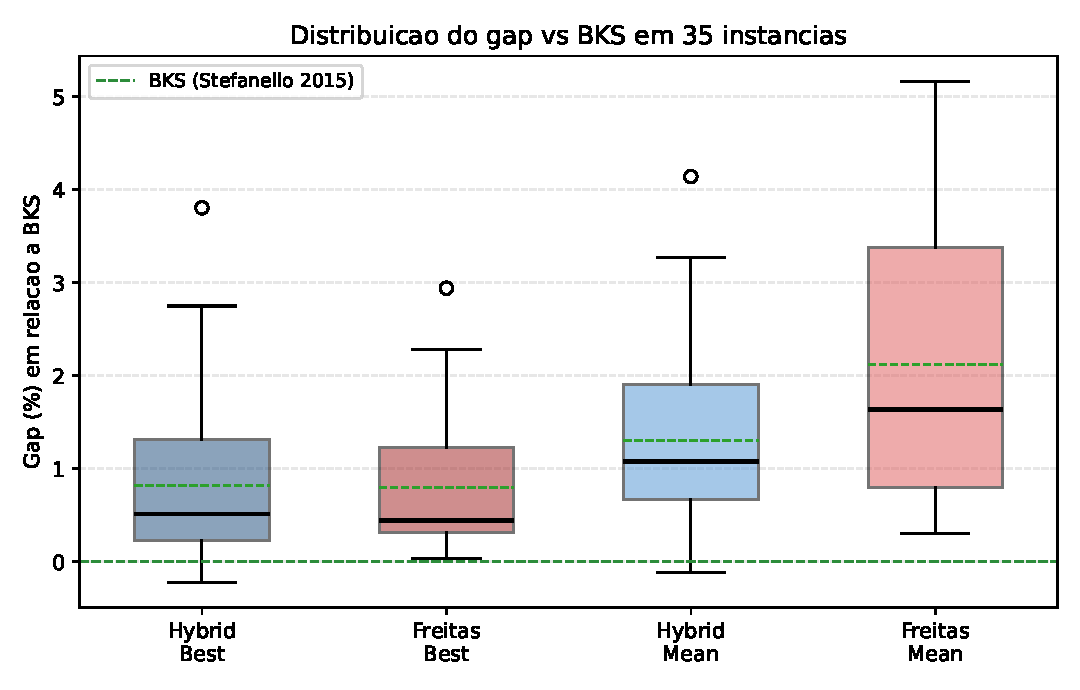
\includegraphics[width=0.78\linewidth]{figuras/boxplot_gap_pct.pdf}
  \caption{Distribuição dos \emph{gaps} percentuais relativos à BKS
  (Equação~\ref{eq:gap}) ao longo das 35 instâncias, para
  $Z_{\mathrm{best}}$ e $Z_{\mathrm{mean}}$ do Hybrid-CS-AILS e do ILS
  de~\cite{freitas2025ils_pmediana}. A linha tracejada indica a BKS.}
  \label{fig:boxplot}
\end{figure}

A vantagem observada em $Z_{\mathrm{mean}}$ é confirmada 
pelo teste pareado de Wilcoxon \emph{signed-rank}, aplicado sobre a
diferença dos \emph{gaps} percentuais com hipótese alternativa
unilateral favorecendo o método proposto: rejeita-se a hipótese nula
ao nível $\alpha = 0{,}05$ ($p = 0{,}011$, 22 vitórias contra 13 em 35
instâncias).



\subsection{Resultados Computacionais: Eficiência Computacional}
\label{subsec:time}

A contribuição central do Hybrid-CS-AILS se evidencia quando qualidade
e tempo de execução são avaliados juntos. A
Figura~\ref{fig:scatter} apresenta, em escala logarítmica no eixo
horizontal, o tempo médio versus o $\overline{\mathrm{gap}}$ relativo à
BKS para cada uma das 35 instâncias e cada um dos quatro métodos. O
Hybrid-CS-AILS é o único método que ocupa a região $T < 10^2$~s com
\emph{gap} inferior a $1\%$, regime no qual se enquadram todas as
configurações testadas das famílias \texttt{lin318}, \texttt{ali535} e
\texttt{u724}. O ILS de~\cite{freitas2025ils_pmediana} é
dominado em praticamente toda a extensão do gráfico: para cada
um de seus pontos existe um ponto do Hybrid-CS-AILS com tempo menor
\emph{e} qualidade melhor. IRMA e GVNS, por sua vez, formam um
agrupamento de pontos de qualidade superior (\emph{gap} próximo de
zero) à custa de tempos que excedem $500$~s mesmo em instâncias de
tamanho intermediário ($n \leq 1000$).

\begin{figure}[!htb]
  \centering
  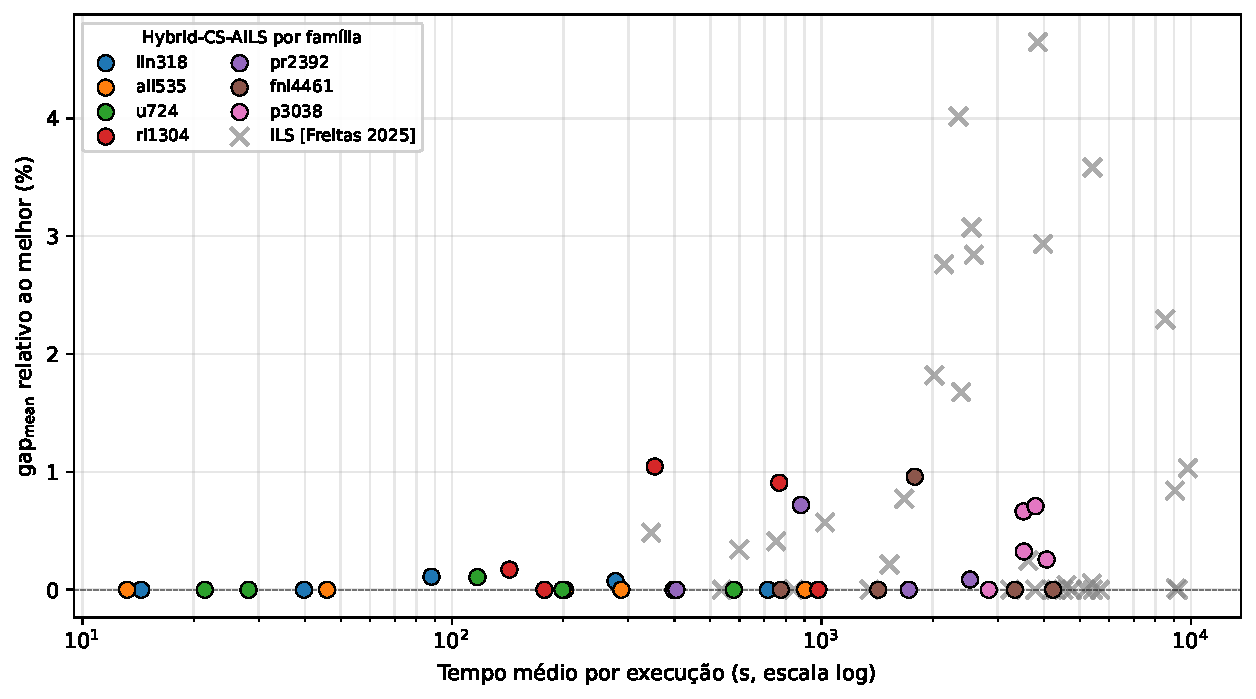
\includegraphics[width=0.85\linewidth]{figuras/time_quality_scatter.pdf}
  \caption{Fronteira tempo $\times$ qualidade.}
  \label{fig:scatter}
\end{figure}

% O ganho em tempo computacional é calculado pela média geométrica das
% razões $T_{\mathrm{baseline}} / T_{\mathrm{Hybrid}}$, por
% instância. O Hybrid-CS-AILS apresenta \emph{speedup} médio de
% $6{,}7\times$ sobre o ILS e o GVNS, e de $2{,}3\times$ sobre a IRMA,
% com ganhos particularmente expressivos em \texttt{ali535}
% ($19{,}0\times$ contra o ILS) e \texttt{u724} ($15{,}4\times$). A
% única família em que o método não é mais rápido que a IRMA é
% \texttt{p3038}, em que a razão $p/n \geq 0{,}3$ leva o \textit{Partial
% Optimizer} a um regime degradado.

A combinação dos dois resultados, qualidade de $Z_{\mathrm{mean}}$ estatisticamente comparável às melhores referências, com tempo de execução de uma ordem de grandeza menor, caracteriza uma região da fronteira tempo $\times$ qualidade ainda não explorada pelas abordagens do PPMC.


\section{Conclusão}
\label{secCon}

Neste trabalho foi proposta uma matheurística híbrida denominada \textit{Hybrid-CS-AILS} para o Problema das p-Medianas Capacitado (PPMC). A abordagem integra mecanismos heurísticos e exatos por meio da combinação entre uma heurística construtiva baseada em GRASP, busca local VND, um framework adaptativo de \textit{Iterated Local Search} e um mecanismo de intensificação seletiva guiado por \textit{Clustering Search}. Diferentemente de abordagens híbridas tradicionais, o método proposto utiliza o \textit{Clustering Search} para auxiliar na decisão de quando aplicar o modelo do PPMC via programação inteira mista, concentrando esforço computacional em regiões promissoras do espaço de busca.

Os experimentos computacionais realizados em 35 instâncias benchmark clássicas do PPMC mostraram que o Hybrid-CS-AILS é capaz de produzir soluções competitivas em qualidade quando comparado a métodos representativos da literatura, incluindo abordagens puramente heurísticas e matheurísticas. Além disso, os resultados evidenciaram elevada estabilidade entre execuções independentes e ganhos expressivos de eficiência computacional, permitindo alcançar soluções de alta qualidade em tempos significativamente menores em diversas famílias de instâncias.

Como perspectivas futuras, pretende-se investigar estratégias de aprendizado para seleção de regiões promissoras do espaço de busca como também avaliar a aplicação da abordagem proposta em outras variantes de problemas de localização de facilidades. 

~\\
\bibliographystyle{sbpo}
\bibliography{bibliography}


\end{document}

